%\motto{Use the template \emph{chapter.tex} to style the various elements of your chapter content.}
\chapter{Grundlegende Quantenalgorithmen}
\label{basic_algorithms} % Always give a unique label
% use \chaptermark{}
% to alter or adjust the chapter heading in the running head

\chapterauthor{Vladimir Alyoshin, Gian-Luca Eberling}

\abstract*{some abstract}

\abstract{some abstract}

\section{Mathematische Grundlagen}

\noindent Im folgenden Abschnitt werden alle relevanten mathematischen Konzepte und Methoden erläutert, die den quantenmechanischen Algorithmen wie Shor's Faktorisierungsalgorithmus oder dem Quantenalgorithmus zum diskreten Logarithmus zugrunde liegen. Dazu zählen grundlegende Verfahren der Zahlentheorie wie der Euklidische Algorithmus und die modulare Arithmetik ebenso wie weiterführende Konzepte wie die Ordnung einer Zahl, die Kettenbruchentwicklung zur Näherung rationaler Zahlen, sowie die Quanten-Fourier-Transformation und die Quanten-Phasenabschätzung. Diese mathematischen Werkzeuge bilden das Fundament für das Verständnis der quantenmechanischen Periodensuche und die effiziente Lösung klassisch schwer lösbarer Probleme.

\subsection{Euklidischer Algorithmus}
Der Euklidische Algorithmus berechnet den größten gemeinsamen Teiler (ggT) zweier Zahlen effizient:
\[
\gcd(a, b) = \gcd(b, a \bmod b)
\]
Dies ist notwendig zur Validierung in Shor's Algorithmus und zur Auswahl der Basis \( a \).

\subsection{Modulare Arithmetik}
In Shor's Algorithmus wird exponentielle modulare Arithmetik verwendet:
\[
f(x) = a^x \bmod N
\]
Die Funktion ist periodisch, was die Grundlage für die Periodenfindung darstellt.

\subsection{Periodizität und Ordnung}
Die Ordnung \( r \) von \( a \bmod N \) ist die kleinste positive ganze Zahl, für die gilt:
\[
a^r \equiv 1 \mod N
\]
Diese Ordnung entspricht der Periode der Funktion \( f(x) \).

\subsection{Kettenbruchentwicklung}
Um aus einer gemessenen Näherung \( j/Q \) eine rationale Zahl \( s/r \) zu finden, verwendet man die Kettenbruchentwicklung:
\[
\frac{j}{Q} \approx \frac{s}{r}
\]
Dabei wird ein Näherungsbruch mit möglichst kleinem Nenner gesucht.

\section{Idee: Primfaktorzerlegung}

Ziel ist es, eine zusammengesetzte Zahl \( N = pq \) effizient zu faktorisieren. Klassische Algorithmen benötigen dazu exponentielle Laufzeit. Shor's Algorithmus nutzt die Periodenstruktur der Funktion
\[
f(x) = a^x \bmod N
\]
um über einen quantenmechanischen Mechanismus – insbesondere die Quanten-Phasenschätzung (QPE) – die Periode \( r \) dieser Funktion effizient zu bestimmen.

\noindent Dabei kommt \textbf{Quanteninterferenz} als zentrales Werkzeug zum Einsatz: Im Quantenalgorithmus wird ein Superpositionszustand über viele mögliche Werte \( x \) erzeugt und durch die Funktion \( f(x) \) moduliert. Dies geschieht durch Anwendung einer unitären Operation \( U_f \), die \( |x\rangle \mapsto |f(x)\rangle \) abbildet. Anschließend wird durch die Quanten-Phasenschätzung in Kombination mit einer inversen Quanten-Fourier-Transformation (iQFT) eine Interferenz zwischen den Zuständen herbeigeführt, die bestimmte periodische Anteile konstruktiv verstärkt und andere destruktiv auslöscht.\\

\noindent Diese Interferenz sorgt dafür, dass bei der anschließenden Messung mit hoher Wahrscheinlichkeit ein Ergebnis nahe einer rationalen Näherung \( s/r \) (mit \( r \) = Periode) beobachtet wird. Der Bruch \( s/r \) wird schließlich mithilfe der Kettenbruchentwicklung in den exakten Wert von \( r \) umgewandelt. Sobald \( r \) bekannt ist und gewisse Bedingungen erfüllt (insbesondere: \( r \) gerade und \( a^{r/2} \not\equiv -1 \bmod N \)), kann man die Teiler von \( N \) effizient mit dem Euklidischen Algorithmus bestimmen:
\[
\gcd(a^{r/2} \pm 1, N)
\]

\noindent So ermöglicht die \textbf{Quanteninterferenz}, zusammen mit der Fourier-Analyse, die entscheidende Extraktion der verborgenen Periodenstruktur, was die Grundlage der Faktorisierung bildet.

\section{Diskreter Logarithmus}

Shor’s Algorithmus kann auch auf das Problem des diskreten Logarithmus angewendet werden. Dieses besteht darin, für eine gegebene Gruppe \( G \), ein Element \( g \in G \) und ein weiteres Element \( h \in G \), die Zahl \( x \) zu finden, sodass:
\[
g^x = h
\]
Auch dieses Problem lässt sich durch Reduktion auf eine Periodensuche effizient mit einem Quantenalgorithmus lösen.

\section{Quanten-Fourier-Transformation}

\subsection{Definition}
Die Quanten-Fourier-Transformation (QFT) auf einem \( n \)-Qubit-System transformiert einen Basiszustand \( \ket{x} \) wie folgt:
\[
\text{QFT}(\ket{x}) = \frac{1}{\sqrt{2^n}} \sum_{k=0}^{2^n-1} e^{2\pi i xk / 2^n} \ket{k}
\]
mit
\begin{itemize}
    \item \( n \): Anzahl der Qubits im Quantenregister, also die Größe des Systems.
    \item \( \ket{x} \): Ein Basiszustand des \( n \)-Qubit-Systems, wobei \( x \in \{0, 1, \ldots, 2^n - 1\} \) eine ganze Zahl ist, die den Basiszustand beschreibt.
    \item \( 2^n \): Die Dimension des Hilbertraums, also die Gesamtanzahl aller Basiszustände für das \( n \)-Qubit-System.
    \item \( k \): Laufindex in der Summe, der ebenfalls von 0 bis \( 2^n - 1 \) reicht und die möglichen Basiszustände nach der Transformation angibt.
    \item \( e^{2 \pi i x k / 2^n} \): Die komplexe Phase, die im Überlagerungszustand die Interferenzmuster erzeugt und so Frequenzinformationen kodiert.
\end{itemize}

\noindent Sie ist zentral für die Phasenerkennung bei der Periodensuche.

\subsection{Komplexität}
Die QFT kann auf einem Quantencomputer effizient in \( \mathcal{O}(n^2) \) durchgeführt werden, im Gegensatz zur klassischen Fourier-Transformation mit \( \mathcal{O}(n 2^n) \).

\section{Quanten-Phasenabschätzung}

\noindent Die Quanten-Phasenabschätzung ermöglicht die Bestimmung der Phase \( \phi \) eines Eigenwerts \( e^{2\pi i \phi} \) einer unitären Matrix \( U \), wobei:
\[
U \ket{u} = e^{2\pi i \phi} \ket{u}
\]
Sie ist ein zentrales Werkzeug zur Ermittlung der Periode \( r \) im Shor-Algorithmus, da man damit die Periode indirekt über eine Phase ablesen kann.


\section{Shor-Algorithmus: Faktorisierung und diskreter Logarithmus}
\label{first:shor-algorithm}
Die klassische Kryptografie basiert auf der Annahme, dass bestimmte mathematische Probleme – wie die Zerlegung großer Zahlen in Primfaktoren – selbst für moderne Supercomputer unlösbar bleiben. Genau hier setzt Shor’s Algorithmus an: 1994 entwickelte der Mathematiker Peter Shor einen Quantenalgorithmus, der dieses Problem effizient lösen kann. Damit stellte er nicht nur eine der zentralen Säulen klassischer Verschlüsselungsverfahren in Frage, sondern zeigte auch das enorme Potenzial von Quantencomputern für konkrete Anwendungen.\\

\noindent In diesem Kapitel erklären wir die Grundidee von Shor’s Algorithmus, zeigen, wie er die periodische Struktur von Funktionen mithilfe der Quanten-Fourier-Transformation nutzt, und machen deutlich, warum seine Effizienz klassisch nicht erreichbar ist. Ziel ist es, die mathematischen Grundlagen verständlich zu machen und Schritt für Schritt zur Quantenlösung des Faktorisierungsproblems zu führen.\\


\subsection{Ablauf des Shor-Algorithmus zur Faktorisierung}

\noindent
Ziel ist es, eine zusammengesetzte Zahl \( N = pq \) in ihre Primfaktoren \( p \) und \( q \) zu zerlegen. Dazu nutzt Shor's Algorithmus einen Quantencomputer zur Berechnung der Periode einer bestimmten Funktion. Der Algorithmus gliedert sich in einen klassischen und einen quantenmechanischen Teil.

\subsubsection*{Schritt 1: Auswahl einer zufälligen Basis}
Wähle eine ganze Zahl \( a \) mit:
\[
1 < a < N \quad \text{und} \quad \gcd(a, N) = 1
\]
Falls \( \gcd(a, N) > 1 \), wurde bereits ein echter Teiler von \( N \) gefunden.

\subsubsection*{Schritt 2: Reduktion auf das Periodenproblem}
Definiere die Funktion
\[
f(x) = a^x \bmod N
\]
Die Funktion \( f(x) \) ist periodisch mit einer Periode \( r \), sodass:
\[
a^r \equiv 1 \mod N
\]
Die Suche nach der kleinsten solchen Zahl \( r \) ist das zentrale Problem, das der Quantencomputer löst.

\subsubsection*{Schritt 3: Periodenfindung mit einem Quantencomputer}

\begin{enumerate}
  \item[3.1] \textbf{Initialisierung:}  
  Zwei Register werden initialisiert mit dem Zustand:
  \[
  \ket{0}^{\otimes n} \otimes \ket{1}
  \]

  \item[3.2] \textbf{Hadamard-Transformation:}  
  Auf das erste Register wird die Hadamard-Transformation angewendet, um eine Superposition zu erzeugen:
  \[
  \frac{1}{\sqrt{Q}} \sum_{x=0}^{Q-1} \ket{x} \otimes \ket{1}
  \]
  
  Dabei ist:
  \begin{itemize}
    \item \( n \): Anzahl der Qubits im ersten Register.
    \item \( Q = 2^n \): Anzahl der möglichen Zustände im ersten Register
    \item \( x \): Laufvariable über alle Basiszustände von \( \ket{0} \) bis \( \ket{Q-1} \).
    \item \( \ket{1} \): Anfangszustand des zweiten Registers, auf das später die modulare Exponentiation angewendet wird.
  \end{itemize}

  Durch die Hadamard-Gates wird das Register in eine Superposition gebracht, in der alle \( Q \) Basiszustände gleichwahrscheinlich sind. Diese Superposition ist notwendig, um später durch die Phaseninterferenz Information über die Periode der Funktion zu extrahieren.\\

  \item[3.3] \textbf{Modulare Exponentiation:}  
  Eine kontrollierte Operation berechnet:
  \[
  \ket{x} \otimes \ket{1} \rightarrow \ket{x} \otimes \ket{a^x \bmod N}
  \]

  \item[3.4] \textbf{Inverse Quanten-Fourier-Transformation (iQFT):}  
  Auf das erste Register wird die iQFT angewendet, um Periodeninformationen in der Amplitudenverteilung zu kodieren.\\

  \item[3.5] \textbf{Messung:}  
  Das erste Register wird gemessen und ergibt einen Wert \( j \), der näherungsweise gilt:
  \[
  \frac{j}{Q} \approx \frac{s}{r}
  \]

  \item[3.6] \textbf{Klassische Kettenbruchentwicklung:}  
  Die rationale Näherung \( \frac{j}{Q} \approx \frac{s}{r} \) wird mithilfe einer Kettenbruchentwicklung bestimmt.  
  Dabei sucht man nach einem Bruch \( \frac{s}{r} \), der \( \frac{j}{Q} \) mit kleinem Nenner \( r \) gut approximiert.\\

  \item[3.7] \textbf{Validierung des Kandidaten:}  
  Überprüfe, ob:
  \[
  a^r \equiv 1 \mod N
  \]
  Falls nicht, versuche eine andere Näherung oder starte mit anderem \( a \) neu.
\end{enumerate}

\subsubsection*{Schritt 4: Klassischer Abschluss}
Wenn eine gültige Periode \( r \) gefunden wurde (und \( r \) gerade ist), berechne:
\[
\gcd\left(a^{r/2} - 1,\; N\right) \quad \text{und} \quad \gcd\left(a^{r/2} + 1,\; N\right)
\]
Diese Werte liefern mit hoher Wahrscheinlichkeit echte Teiler von \( N \). Ist das nicht der Fall, beginnt der Algorithmus erneut mit einer anderen Basis \( a \).

\subsubsection*{Zusammenfassung des Verfahrens}
Der Shor-Algorithmus zeigt, wie Quantencomputer periodische Strukturen in Funktionen aufdecken können, die klassisch nur mit exponentiellem Aufwand zu finden wären. Die Kombination aus Quanten-Phasenabschätzung, Fourier-Transformation und Kettenbruchentwicklung ermöglicht eine effiziente Faktorisierung großer Zahlen – ein fundamentaler Angriff auf die Sicherheit klassischer Verschlüsselung.\\

\noindent Die Operationen des Shor's Algorithmus zur Faktorisierung lassen sich wie folgt darstellen:

\begin{algorithm}[H]
\caption{Shor's Algorithmus zur Faktorisierung einer Zahl \( N \)}
\label{algorithm:shor}
\begin{algorithmic}[1]
\Require Eine zusammengesetzte Zahl \( N \) aus zwei unbekannten Primzahlen \( p \) und \( q \)
\Ensure Ein nicht-trivialer Teiler von \( N \)

\State Wähle zufällig eine ganze Zahl \( a \) mit \( 1 < a < N \)
\If{\( \gcd(a, N) \neq 1 \)}
    \State \Return \( \gcd(a, N) \) \Comment{Zufällig gewähltes \( a \) war bereits ein Teiler}
\EndIf

\State \textbf{Bestimme die Periode \( r \) der Funktion \( f(x) = a^x \bmod N \) mittels Quanten-Phasenschätzung:}
\State \hspace{1em} Initialisiere zwei Quantenregister:
\State \hspace{2em} Erstes Register in Superposition über \( x = 0, \ldots, Q-1 \)
\State \hspace{2em} Zweites Register im Zustand \( \ket{1} \)

\State Wende die unitäre Operation \( U_f \colon \ket{x}\ket{1} \mapsto \ket{x}\ket{a^x \bmod N} \) an
\State Wende die inverse Quanten-Fourier-Transformation (iQFT) auf das erste Register an
\State Messe das erste Register, erhalte Näherung des Bruchs \( \frac{s}{r} \)
\State Berechne \( r \) durch Kettenbruchentwicklung aus \( \frac{s}{r} \)

\If{\( r \) ungerade \textbf{oder} \( a^{r/2} \equiv -1 \mod N \)}
    \State \Return \textbf{Fehlschlag – wähle neues \( a \)} und gehe zu Schritt 1 zurück
\EndIf

\State Berechne \( \gcd(a^{r/2} - 1, N) \) und \( \gcd(a^{r/2} + 1, N) \)
\State \Return Einer der berechneten Werte ist ein nicht-trivialer Teiler von \( N \)
\end{algorithmic}
\end{algorithm}

\subsection{Anwendung auf den RSA-Algorithmus}

\noindent
Der RSA-Algorithmus basiert auf der Schwierigkeit, eine große Zahl \( N = pq \) zu faktorisieren. Shor’s Algorithmus bricht diese Sicherheit, indem er in polynomialer Zeit die Faktoren \( p \) und \( q \) bestimmt. Hat ein Angreifer Zugriff auf einen leistungsfähigen Quantencomputer, kann er aus dem öffentlichen Schlüssel die privaten Schlüsselparameter rekonstruieren:
\begin{itemize}
  \item Berechne \( p \) und \( q \) mit Shor.
  \item Berechne \( \phi(N) = (p-1)(q-1) \).
  \item Berechne den privaten Schlüssel \( d \) durch:
  \[
  d \equiv e^{-1} \mod \phi(N)
  \]
\end{itemize}
Dies zeigt, dass RSA bei hinreichend großen Quantencomputern als unsicher gelten muss.

\subsection{Anwendung auf das diskrete Logarithmusproblem}

Shor’s Algorithmus kann nicht nur die Primfaktorzerlegung beschleunigen, sondern auch das diskrete Logarithmusproblem effizient lösen. Dieses Problem ist die Grundlage vieler kryptografischer Verfahren wie Diffie-Hellman oder ElGamal. \\

\noindent Das Ziel ist, für gegebenes \( a, b \) in einer Gruppe \( \mathbb{Z}_p^* \) den Exponenten \( x \) zu finden, sodass:
\[
a^x \equiv b \mod p
\]

\noindent Shor’s Algorithmus reduziert das Problem auf die Periodensuche einer geeigneten Funktion durch Quanten-Phasenabschätzung, ähnlich wie bei der Faktorisierung. Dabei wird aus der Überlagerung von Zuständen und anschließender Quanten-Fourier-Transformation die gesuchte Periode extrahiert, die Rückschlüsse auf den Exponenten \( x \) erlaubt.\\

\begin{algorithm}[H]
\caption{Quantenalgorithmus zur Bestimmung des diskreten Logarithmus \( x \) aus \( g^x \equiv h \bmod p \)}
\begin{algorithmic}[1]
\Require Eine Primzahl \( p \), eine erzeugende Basis \( g \in \mathbb{Z}_p^* \) und ein Element \( h \in \mathbb{Z}_p^* \), sodass \( h = g^x \bmod p \)
\Ensure Der Exponent \( x \)

\State Setze eine ausreichend große Zahl \( Q = 2^n \) mit \( Q > p^2 \)
\State Initialisiere zwei Quantenregister:
\State \hspace{1em} Erstes Register: Superposition über \( x = 0, \ldots, Q-1 \)
\State \hspace{1em} Zweites Register: Zustand \( \ket{1} \)
\State Wende die unitäre Operation \( U_g \colon \ket{x}\ket{1} \mapsto \ket{x}\ket{g^x \bmod p} \) an
\State Wende die inverse Quanten-Fourier-Transformation (iQFT) auf das erste Register an
\State Messe das erste Register, erhalte Näherung des Bruchs \( \frac{s}{r} \)
\State Berechne \( r \) durch Kettenbruchentwicklung aus \( \frac{s}{r} \)
\If{\( r \) ist ungültig oder keine passende Ordnung gefunden}
  \State \textbf{Gehe zu Schritt 2 zurück.}
\EndIf
\State Führe klassische Nachbearbeitung durch, um \( x \) aus \( r \), \( s \) und \( h \) zu bestimmen
\State \Return \( x \)
\end{algorithmic}
\end{algorithm}

\subsection{Shor's Faktorisierung Algorithmus am Beispiel \( N = 15 \)}
Finde einen nicht-trivialen Teiler von \( N = 15 \), also \( p = 3 \) oder \( q = 5 \), mithilfe von Shor's Algorithmus.

\subsection*{Schritt 1: Wahl einer Zufallszahl}
Wähle eine ganze Zahl \( a \) mit \( 1 < a < N \).  
Wir wählen \( a = 2 \).

Berechne den größten gemeinsamen Teiler:
\[
\gcd(2, 15) = 1
\]
Da \( \gcd(a, N) = 1 \), fahren wir fort.

\subsection*{Schritt 2: Periodenbestimmung via Quantenalgorithmus}

\subsubsection*{Teil a) Initialisierung}
Verwende zwei Register:
\begin{itemize}
    \item Erster Register: \( n \)-Qubits mit \( 2^n \geq N^2 \). Für Demonstration genügt \( n = 4 \).
    \item Zweiter Register: \( m = \lceil \log_2(N) \rceil = 4 \)
\end{itemize}

Anfangszustand:
\[
\ket{\psi_0} = \ket{0}^{\otimes 4} \otimes \ket{1}
\]

\subsubsection*{Teil b) Hadamard-Transformation}
Wende auf jedes Qubit im ersten Register ein Hadamard-Gate an:
\[
\ket{\psi_1} = \frac{1}{\sqrt{16}} \sum_{x=0}^{15} \ket{x} \otimes \ket{1}
\]

\subsubsection*{Teil c) Modulare Exponentiation}
Wende die unitäre Transformation \( U_f \) an, die definiert ist als:
\[
U_f: \ket{x}\ket{1} \mapsto \ket{x}\ket{2^x \mod 15}
\]

Beispiele:
\begin{align*}
2^0 \mod 15 &= 1 \\
2^1 \mod 15 &= 2 \\
2^2 \mod 15 &= 4 \\
2^3 \mod 15 &= 8 \\
2^4 \mod 15 &= 1 \\
2^5 \mod 15 &= 2 \\
2^6 \mod 15 &= 4 \\
2^7 \mod 15 &= 8 \\
&\vdots
\end{align*}

Periode \( r = 4 \).

\subsubsection*{Teil d) Inverse Quanten-Fourier-Transformation (iQFT)}
Wende die inverse QFT auf das erste Register an.

Da wir wissen, dass die Periode $r = 4$ ist, erhalten wir nach idealer iQFT einen Superpositionszustand, bei dem die Amplituden auf den Vielfachen von $\frac{2^n}{r} = \frac{16}{4} = 4$ konzentriert sind (bei $n = 4$ Qubits im ersten Register):

\[
|\psi_3\rangle = \frac{1}{2} \sum_{k=0}^{3} |k \cdot 4\rangle \otimes |2^x \bmod 15\rangle
\]

Konkret also:

\[
|\psi_3\rangle = \frac{1}{2}\left( |0\rangle + |4\rangle + |8\rangle + |12\rangle \right) \otimes |2^x \bmod 15\rangle
\]

Die Messung des ersten Registers ergibt dann mit gleicher Wahrscheinlichkeit einen der Werte:

\[
\boxed{0,\ 4,\ 8,\ 12}
\]

Alle diese Werte sind Vielfache von $4$, was ein Hinweis auf die Periode $r$ ist. Nach der Messung verwenden wir eine Kettenbruchentwicklung auf den gemessenen Wert $s$ (z.B. $s = 4$) geteilt durch $2^n = 16$, um $r \approx \frac{2^n}{s}$ zu rekonstruieren.

\subsubsection*{Teil e) Messung}
Messe das erste Register. Angenommen, das Ergebnis ist \( x = 4 \).

Damit gilt:
\[
\frac{x}{2^n} = \frac{4}{16} = \frac{1}{4} \Rightarrow r = 4
\]

\subsection*{Schritt 3: Klassischer Teil – Faktorenberechnung}

\begin{itemize}
    \item Prüfe, ob \( r \) gerade: \( r = 4 \Rightarrow \text{ja} \)
    \item Berechne:
    \[
    a^{r/2} = 2^2 = 4
    \]
    \item Bestimme:
    \[
    \gcd(4 - 1, 15) = \gcd(3, 15) = 3
    \]
    \[
    \gcd(4 + 1, 15) = \gcd(5, 15) = 5
    \]
\end{itemize}

\subsection*{Schritt 4: Ergebnis}
Wir haben erfolgreich die Primfaktoren gefunden:
\[
15 = 3 \times 5
\]

\section{Grover-Algorithmus: Quantum-Suche}
\label{sec:grover-algorithm}
In der Informatik zählt die Datenverarbeitung zu den gefragtesten Aufgaben. In der heutigen Zeit ist die Möglichkeit, große Datenmengen zu durchsuchen — insbesondere unstrukturierte Daten — ein wesentlicher Aspekt der Datenanalyse. Um dies zu veranschaulichen, betrachten wir folgendes Beispiel:\\ 

Angenommen, wir möchten einen bestimmten Kunden in der Datenbank eines Online-Shops finden (unter der Annahme, dass die Datenbank nicht indexiert ist). Bei Verwendung eines klassischen Computers benötigen wir im schlechtesten Fall $N$ Iterationen, wobei $N$ die Anzahl der Zeilen in der Tabelle darstellt. Im durchschnittlichen Fall sind etwa $N/2$ Operationen erforderlich. Das bedeutet, dass alle Elemente der Tabelle durchlaufen werden müssen, sofern uns die genaue Position des gesuchten Kunden nicht bekannt ist — bis dieser schließlich gefunden wird.\\

Wenn jedoch unsere Datenbank auf Quantenberechnungen basiert, können wir Quanten-Suchalgorithmen wie den Grover-Algorithmus einsetzen. In diesem Fall lässt sich das gesuchte Element mit etwa $\sqrt{N}$ Operationen finden. Zwar führt dieser Algorithmus nicht zu einer exponentiellen Beschleunigung der Suche und muss häufig mehrfach iterativ aufgerufen werden, dennoch stellt die quadratische Laufzeit bereits eine bedeutende Optimierung dar.

\subsection{Grundlagen: Unstrukturiertes Suchproblem}
Bevor wir uns dem Grover-Algorithmus zuwenden, betrachten wir folgendes Beispiel: Stellen wir uns vor, auf dem Tisch liegen vier Spielkarten verdeckt. Eine dieser vier Karten ist die Pik-Dame, und unsere Aufgabe besteht darin, sie zu finden. Wie viele Karten müssen wir im Durchschnitt aufdecken, um die Pik-Dame zu identifizieren? Im besten Fall finden wir die gesuchte Karte bereits beim ersten Versuch. Im schlechtesten Fall müssen wir drei Karten umdrehen — wenn keine von ihnen die Pik-Dame ist, dann bleibt nur noch die vierte, nicht aufgedeckte Karte als einzig mögliche Lösung. Im Durchschnitt müssen wir 2{,}25 Karten aufdecken, um die Pik-Dame zu finden.\\

Formulieren wir nun das Beispiel um: Anstelle von Spielkarten betrachten wir eine binäre Reihenfolge natürlicher Zahlen — nämlich $00$, $01$, $10$ und $11$. Nehmen wir an, die Pik-Dame entspricht dabei der Zahl $11$. Wir definieren eine Funktion $f$, die den Wert $1$ zurückgibt, wenn das Eingabemuster $11$ ist, und $0$ in allen anderen Fällen. Somit lässt sich das Problem wie folgt formal ausdrücken:

\begin{definition}[Unstrukturiertes Suchproblem]
Sei $f\colon \{0, 1\}^n \rightarrow \{0, 1\}$ eine abstrakte Funktion mit $f(x) \in \{0, 1\}$. Gesucht ist ein Wert $x$, sodass $f(x) = 1$, falls ein solcher Wert existiert; andernfalls soll das Ergebnis $0$ sein.
\end{definition}

Die Komplexität des unstrukturierten Suchproblems ergibt sich daraus, wie viele Iterationen der Funktion erforderlich sind, um das gesuchte Element zu finden. Wir benötigen im schlechtesten Fall $N - 1$ Funktionsauswertungen, wobei $N = 2^n$ gilt. Auf diese Weise prüfen wir alle möglichen Eingaben. Ähnlich wie im Beispiel mit den Karten entspricht $N$ dem letzten Element, vorausgesetzt, die vorherigen wurden bereits geprüft. Der Grover-Algorithmus kann dieses Problem jedoch deutlich schneller lösen und erreicht dabei eine quadratische Laufzeitverbesserung.\\

Jedoch repliziert der Grover-Algorithmus noch ein Suchproblem. Wie wir im Beispiel mit den Spielkarten gesehen haben, müssen wir Karte für Karte umdrehen, um zu prüfen, ob es die gesuchte Karte ist oder nicht. Dieser Prozess ist iterativ und wird durch das \textit{heuristische Suchproblem} beschrieben:

\begin{definition}[Heuristisches Suchproblem]
Gegeben sei die Möglichkeit, einen probabilistischen „Rate“-Algorithmus \( A \) auszuführen, und eine „Prüf“-Funktion \( f \), sodass

\[
\Pr\left[ A \text{ gibt } w \text{ aus, sodass } f(w) = 1 \right] = \varepsilon,
\]
\end{definition}

Eine Möglichkeit, das heuristische Suchproblem klassisch zu lösen, besteht darin, den Algorithmus \( A \) wiederholt auszuführen und jedes Ergebnis mit der Funktion \( f \) zu überprüfen. Dies führt zu durchschnittlich \( O\left(\frac{1}{\varepsilon}\right) \) Auswertungen von \( f \). In der nächsten Sektion werden wir sehen, wie der Grover-Algorithmus dieses Verfahren implementiert.

\subsection{Aufbau von dem Grover Algorithmus}

Um den Grover-Algorithmus vollständig zu verstehen, ist es wichtig, zunächst die grundlegenden Quantenoperationen zu begreifen. Lov Grover führte die folgende Definition für eine bestimmte Klasse von Operationen ein.\cite[1-2{lavor_grovers_2008}


\begin{definition}[Unitäre Operationen]
Quantenmechanische Operationen, die in kontrollierter Weise ausgeführt werden können, sind \emph{unitäre Operationen}, welche in jedem Schritt auf eine kleine Anzahl von Qubits wirken.
\end{definition}

Der Grover-Algorithmus basiert auf einer Folge solcher unitären Operationen, die auf einen reinen Anfangszustand angewendet werden. Diese Operationen dienen dazu, die Wahrscheinlichkeit des gesuchten Ergebnisses zu verstärken. Am Ende des Algorithmus erfolgt eine Messung des resultierenden Zustands. Diese Messung projiziert das überlagerte Quantensystem auf einen klassischen Zustand, der mit hoher Wahrscheinlichkeit die Lösung des zugrunde liegenden Suchproblems enthält.\\

Lov Grover definierte die folgenden unitären Operationen als zentrale Bestandteile seines Algorithmus:

\begin{enumerate}
    \item \textbf{Initialisierung in einen Superpositionszustand:} 
    Die erste Operation besteht darin, ein Quantenregister mit $n$ Qubits (entsprechend $N = 2^{n}$ möglichen Zuständen) in einen Zustand zu überführen, in dem alle Basiszustände mit der gleichen Wahrscheinlichkeit auftreten – also eine \textit{Gleichverteilung}. Die \textit{Gleichverteilung} wird dadurch erreicht, dass die Amplituden aller Zustände gleich sind. Wenn das System anfangs im Zustand $\ket{0}^{\otimes n}$ ist (alle Qubits auf 0), dann erzeugen wir durch Anwendung der Hadamard-Transformation auf jedes Qubit die Superposition:

$$
\ket{\psi_0} = \frac{1}{\sqrt{N}} \sum_{x=0}^{N-1} \ket{x}
$$

Dies ist die gleichmäßige Superposition über alle möglichen Zustände $\ket{x}$ mit $x \in {0, \ldots, N-1}$.\\
    \item \textbf{Walsch-Hadamard Transformation}: Hadamard Transformation ist eine wichtige Quantummechanische Operation, die durch eine Operation $H$ definiert ist. Diese Operation wird auf ein einzelnes Qubit angewendet und wird durch die folgende Matrix dargestellt:
    $$
H = \frac{1}{\sqrt{2}} \begin{pmatrix}
1 & 1 \\
1 & -1 \\
\end{pmatrix}
$$
Ein Qubit im Zustand \( \lvert 0 \rangle \) wird in eine Superposition der beiden Zustände überführt: \( \left( \frac{1}{\sqrt{2}}, \frac{1}{\sqrt{2}} \right) \). Die Wirkung auf die Basiszustände ist:

$$
H\ket{0} = \frac{1}{\sqrt{2}}(\ket{0} + \ket{1}), \quad H\ket{1} = \frac{1}{\sqrt{2}}(\ket{0} - \ket{1})
$$
Wendet man $H$ auf jedes der $n$ Qubits an, so entsteht eine Transformation $H^{\otimes n}$, die eine $2^n \times 2^n$-Matrix darstellt.
Besonders interessant ist, dass das Vorzeichen (also die Phase) des Amplitudenwertes nach der Hadamard-Transformation vom Skalarprodukt der Eingabe- und Ausgabebits abhängt:

$$
\text{Vorzeichen} = (-1)^{x \cdot y}
$$

Dabei ist $x \cdot y$ das bitweise Skalarprodukt der $n$-Bit-Binärzahlen $x$ und $y$.\\

    \item \textbf{Selektive Phasenrotation:} Die dritte elementare Operation ist die selektive Phasenrotation der Amplitude in bestimmten Zuständen. Die Transformation, die dies für ein Zwei-Zustands-System beschreibt, hat die Form:

    $$
R = \begin{pmatrix}
e^{i\phi_1} & 0 \\
0 & e^{i\phi_2}
\end{pmatrix}
$$

wobei \( \phi \) eine beliebige reelle Zahl ist. Es ist zu beachten, dass – im Gegensatz zur Walsh-Hadamard-Transformation und anderen Zustandsübergangsmatrizen – die Wahrscheinlichkeit in jedem Zustand gleich bleibt, da das Quadrat des Betrags der Amplitude in jedem Zustand unverändert bleibt.
Im Grover-Algorithmus wird die Phasenrotation speziell dafür genutzt, um den gesuchten Zustand $\ket{x\_{\text{target}}}$ zu markieren, indem dessen Amplitude mit $-1$ multipliziert wird, während alle anderen Zustände unverändert bleiben:

$$
\ket{x} \mapsto 
\begin{cases}
- \ket{x}, & \text{wenn } x = x_{\text{target}} \\
\ket{x}, & \text{sonst}
\end{cases}
$$

\end{enumerate}

Zusammenfassend lässt sich einfach sagen: Der Grover-Algorithmus verwendet diese Operationen, um pro Iteration zwei Schritte auszuführen:
\begin{enumerate}
  \item Vorzeichenumkehr der Wahrscheinlichkeitsamplitude des gesuchten Elements.
  \item Verstärkung der Wahrscheinlichkeitsamplitude.
\end{enumerate}

Mit dem Verständnis der oben genannten unitären Operationen lässt sich der Grover-Algorithmus durch die folgenden Schritte beschreiben:

\begin{algorithm}[H]
\label{alg:grover}
\caption{Grover-Suchalgorithmus}
\begin{algorithmic}[1]
\State Erzeuge ein Register aus \( n \) Qubits im Zustand \( \ket{0}^{\otimes n} \).
\State Wende die Hadamard-Operation \( H \) auf jedes Qubit an, um eine Superposition zu erzeugen.
\Repeat
  \State\textbf{Oracle:}
  \State \hspace{1em} Sei das System im Zustand \( \ket{x} \).
  \If{ \( f(x) = 1 \) }
    \State Rotiere die Phase von \( \ket{x} \) um \( \pi \) Radiant.
  \Else
    \State Belasse \( \ket{x} \) unverändert.
  \EndIf
  \State Wende die Grover-Diffusionstransformation $D$ an.
  \State Messe das Register zur Bestimmung des gesuchten Index.
\If{das Ergebnis ist keine gültige Lösung}
  \State Gehe zu Schritt 3 zurück.
\EndIf
\Until{eine gültige Lösung mit hoher Wahrscheinlichkeit gefunden wurde}
\end{algorithmic}
\end{algorithm}

Ein entscheidender Schritt in diesem Algorithmus ist die \textit{Grover-Diffusions\-transformation}, die wesentliche Änderungen an den Amplituden bewirkt. Nämlich, sie verstärkt gezielt die Amplitude des gesuchten Zustands. Um Diffusionstransformation zu verstehen, erwähnt Grover in seiner Arbeit das Konzept der \textit{lokalen Übergangsmatrizen} ein.

\begin{definition}[Lokale Übergangsmatrizen]
Lokale Übergangsmatrizen sind Matrizen, in denen nur eine konstante Anzahl von Elementen in jeder Spalte ungleich null ist.
\end{definition}

Anschließend führt Grover den Begriff der Diffusionstransformation ein:

\begin{definition}[Grover-Diffusionstransformation]
\( D \) ist keine lokale Übergangs\-matrix, da es Übergänge von jedem Zustand zu allen \( N \) Zuständen gibt:
$$
D_{ij} = 
\begin{cases}
\frac{2}{N}, & \text{wenn } i \ne j \\
1 - \frac{2}{N}, & \text{wenn } i = j
\end{cases}
$$
Unter Verwendung der Walsh-Hadamard-Transformationsmatrix kann \( D \) als Produkt von drei lokalen unitären Transformationen implementiert werden:
$$
D = H \cdot R \cdot H
$$
Hierbei sind:
\begin{itemize}
\item $H$: Die \textbf{Hadamard-Transformation} auf allen $n$ Qubits.
\item $R$: Eine \textbf{Phaseninversionsmatrix} (Phasenrotationsmatrix), die nur den Zustand $\ket{0}^{\otimes n}$ (alle Qubits sind 0) mit $-1$ multipliziert, alle anderen Zustände bleiben unverändert.
\end{itemize}
\end{definition}

Alle für den Grover-Algorithmus nötigen Operationen bestehen aus nur zwei fundamentalen Bausteinen - \textbf{Hadamard-Gates} und \textbf{Phaseninversionen}. Dadurch ist der Grover-Algorithmus im Vergleich zu anderen Quantenalgorithmen – z.,B. solchen wie Shor's Algorithmus \ref{algorithm:shor}, die eine Quantum Fourier-Transformation(QFT) benötigen – relativ einfach zu implementieren. In der nächsten Sektion betrachten wir den Grover-Algorithmus Implementierung Schritt für Schritt anhand eines konkreten Beispiels.

\subsection{Beispielanwendung von Grover-Algorithmus}

Um ein Beispiel für die Funktionsweise des Grover-Algorithmus zu betrachten, ohne den Überblick zu verlieren, analysieren wir ein kleineres Beispiel – basierend auf drei Qubits. Wir greifen erneut auf das Beispiel mit den Karten zurück: Nehmen wir an, alle vier Karten sind mit Hilfe von zwei Qubits kodiert. Dann erhalten wir die folgenden Daten: 00, 01, 10 und 11. Den dritten Qubit werden wir als Hilfsqubit  verwenden – mit seiner Hilfe können wir die gesuchte Karte durch Multiplikation mit -1 markieren. Anschließend betrachten wir die Anwendung des Grover-Algorithmus auf dieses Beispiel.\\

Das Quantenschaltbild sieht folgendermaßen aus:
\begin{figure}[h!]
    \centering
    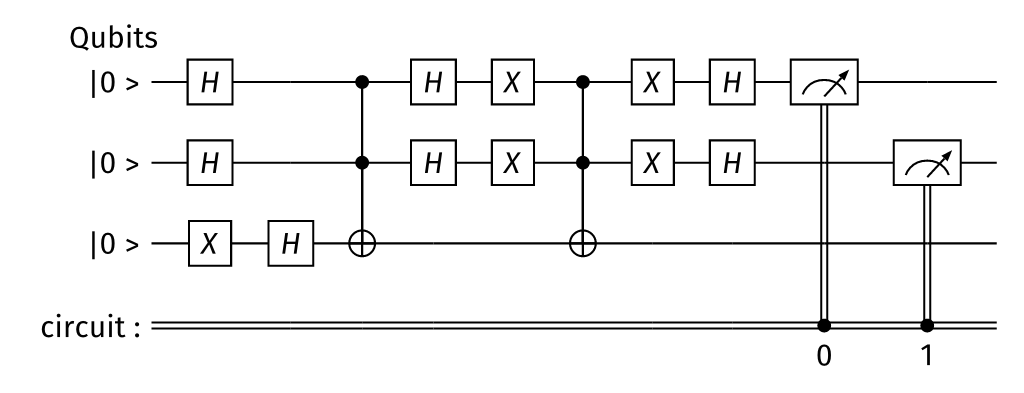
\includegraphics[width=0.9\textwidth]{images/basic-algorithms/3-qubits-grover.png}
    \caption{Grover-Algorithmus für $n=2$ (das gesuchte Element - $11$)}
    \label{fig:grover-three-bits}
\end{figure}

Zu Beginn, noch vor dem Start der Iterationen, müssen alle Qubits – einschließlich des Hilfsqubits – in eine Superposition gebracht werden. Dabei sollen sich zu Anfang alle Qubits im Zustand $0$ befinden, mit Ausnahme des Hilfsqubits, der vor der Hadamard-Operation in den Zustand $1$ gesetzt wird.\\

Nach Anwendung des Hadamard-Gatters befindet sich das Hilfsqubit somit im Zustand $\frac{1}{\sqrt{2}}(|0\rangle - |1\rangle)$, während alle übrigen Qubits den Zustand $\frac{1}{\sqrt{2}}(|0\rangle + |1\rangle)$ annehmen.

Anschließend beginnen die Iterationen. Jede Iteration besteht aus zwei Phasen. Die erste Phase ist die Anwendung der Orakelfunktion. Wie es in Grover-Algorithmus \ref{alg:grover} vorgestellt wurde, handelt es sich um eine Funktion, die effizient bestimmen kann, welcher Index dem gesuchten Element entspricht. Zwar kann diese Funktion den Index nicht direkt mitteilen, jedoch ist sie in der Lage, diesen Zustand mit einem Minuszeichen zu markieren.

Um das Funktionsprinzip des Algorithmus in diesem Beispiel besser zu verstehen, definieren wir eine vereinfachte Orakelfunktion manuell. Dabei ist zu beachten, dass die tatsächliche Orakelfunktion in der Praxis spezifisch an die jeweilige Aufgabe angepasst ist und daher möglicherweise anders implementiert wird. Auf die konkrete technische Realisierung der Orakelfunktion zur Datensuche gehen wir hier nicht ein, da dies den grundlegenden Ablauf von Grovers Algorithmus nicht beeinflusst.

Für das Verständnis des Grover-Algorithmus ist es entscheidend nachzuvollziehen, wie sich die Zustände der Qubits verändern, bis zum Zeitpunkt der Messung, die schließlich den gesuchten Index liefert.In diesem Beispiel haben wir als das gesuchte Index $11$ definiert - so wie es in dem Beispiel von Karten gab. Das bedeutet, dass die Messung am Ende genau dieses Ergebnis liefern soll. Wir modellieren daher ein Orakel, das genau diesen Index markiert. Als solche Orakelfunktion eignet sich das Toffoli-Gatter ($CCNOT$), das bei Ansteuerung beider Kontrollqubits mit dem Wert $1$ ein $X$-Gatter auf das Zielqubit – in diesem Fall das Hilfsqubit – anwendet:

\begin{definition}[Toffoli-Gatter]
\label{def:toffoli}
Das Toffoli-Gatter, auch bekannt als $CCNOT$-Gatter (für „controlled-controlled-not“), ist eine Erweiterung des bekannten $CNOT$-Gatters mit zwei Steuerbits und einem Zielbit. Das bedeutet: Das Zielbit (das dritte Bit) wird genau dann invertiert, wenn sowohl das erste als auch das zweite Steuerbit den Wert $1$ haben.\ref{toffoli}
\end{definition}

Das Toffoli-Gatter sieht folgendermaßen aus:
\begin{figure}[H]
    \centering
    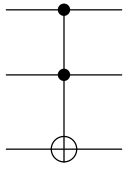
\includegraphics[width=0.2\textwidth]{images/basic-algorithms/toffoli.png}
    \caption{$CCNOT$ - Toffoli-Gatter}
    \label{fig:toffoli-gate}
\end{figure}

 Für die Zustände der oberen Qubits, die die Indizes $00$, $01$ und $10$ codieren, bleibt das Toffoli-Gatter ohne Wirkung – der Hilfsqubit verbleibt in dem Zustand $\frac{1}{\sqrt{2}}(|0\rangle - |1\rangle)$.\\

 Erst beim Index $11$ wird das Gatter aktiv: Es wendet das $X$-Gatter auf den Hilfsqubit an, wodurch dieser den Zustand $\frac{1}{\sqrt{2}}(|1\rangle - |0\rangle)$ annimmt\ref{def:toffoli}. Dieser lässt sich äquivalent als $-\frac{1}{\sqrt{2}}(|0\rangle - |1\rangle)$ schreiben – das Minuszeichen erscheint also vor dem gesamten Zustand.\\

 Dieses Minuszeichen bezieht sich nicht nur auf den Hilfsqubit, sondern auf den gesamten Zustand, der dem Index $11$ entspricht. Daher kann man den Hilfsqubit als unverändert betrachten und das Vorzeichen dem Zustand der oberen Qubits zuordnen. Damit ist der Index $11$ als der gesuchte Zustand mit einem Minus gekennzeichnet. Anders ausgedrückt: Die Orakelfunktion transformiert den Zustand $|11\rangle\,|q_{\text{3}}\rangle$ in $-|11\rangle\,|q_{\text{3}}\rangle$, wobei $|q_{\text{3}}\rangle$ den Zustand des Hilfsqubits bezeichnet.

Den Zustand des Quantensystems nach Anwendung des Orakels können wir folgendermaßen ausdrücken (der Hilfsqubit steht in der rechten Klammer):

$$
|\psi\rangle = \frac{1}{2\sqrt{2}} (|00\rangle + |01\rangle + |10\rangle - |11\rangle)(|0\rangle - |1\rangle)
$$

Damit ist der erste Teil der ersten Iteration abgeschlossen. Der gesuchte Index wurde markiert, aber eine sofortige Messung der Qubits würde keinen Nutzen bringen – das Minuszeichen zeigt sich im Messergebnis nicht. Außerdem würde der Index $11$ mit einer Wahrscheinlichkeit von nur $0{,}25$ erscheinen – genau wie alle anderen Indizes.

Um die weiteren Schritte besser zu verstehen, stellen wir uns die erste Hälfte des Algorithmus grafisch als Zustandsvektor vor. Die horizontale Achse definieren wir als Einheitsvektor, der alle Zustände der Superposition enthält – mit Ausnahme des gesuchten Zustands. Die vertikale Achse steht für den gesuchten Basiszustand.

Der Zustandsvektor $c$, also der Zustand des Systems vor der ersten Iteration, ist eine Linearkombination dieser beiden Basisvektoren entlang der horizontalen und vertikalen Achse.\ref{fig:initial-grover-three-qubits}

\begin{figure}[H]
    \centering
    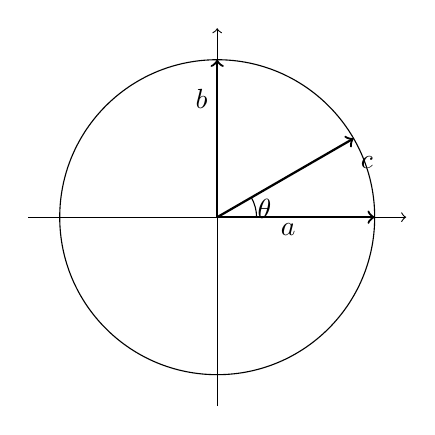
\begin{tikzpicture}[scale=2]
    % Draw coordinate axes
    \draw[->] (-1.2, 0) -- (1.2, 0); % x-axis
    \draw[->] (0, -1.2) -- (0, 1.2); % y-axis

    % Draw the unit circle
    \draw (0,0) circle(1);

    % Angle theta
    \draw[->, thick] (0,0) -- (0.866,0.5); % hypotenuse (c)
    \node at (0.95,0.35) {$c$};

    % Projection on x-axis (a)
    \draw[->, thick] (0,0) -- (1,0);
    \node at (0.45,-0.08) {$a$};

    % Projection on y-axis (b)
    \draw[->, thick] (0,0) -- (0,1);
    \node at (-0.1,0.75) {$b$};

    % Angle label θ
    \draw (0.25,0) arc[start angle=0,end angle=30,radius=0.25];
    \node at (0.3,0.05) {$\theta$};
\end{tikzpicture}
    \caption{Der initiale Zustand des Systems}
    \label{fig:initial-grover-three-qubits}
\end{figure}

Im Fall dieses Beispiels (ein System aus zwei Qubits mit dem gesuchten Index $11$) lässt sich der Zustandsvektor $c$ durch die Koordinaten $x$ und $y$ wie folgt darstellen:

$$
\frac{1}{2}(|00\rangle + |01\rangle + |10\rangle + |11\rangle) = x \cdot \frac{1}{\sqrt{3}}(|00\rangle + |01\rangle + |10\rangle) + y \cdot |11\rangle
$$

\noindent Aus dieser Gleichung ergibt sich: $x = \frac{\sqrt{3}}{2}$ und $y = \frac{1}{2}$.\\

Anhand dieser Koordinaten erkennt man, dass der Winkel $\theta$ zwischen dem Vektor $c$ und der horizontalen Achse gleich $\frac{\pi}{6}$ ist. Vorausblickend lässt sich sagen: Unser Ziel ist es, diesen Winkel auf $\frac{\pi}{2}$ (oder zumindest in dessen Nähe) zu bringen – also den Zustand nahezu vollständig in Richtung des gesuchten Basiszustands zu drehen, sodass bei der anschließenden Messung mit hoher Wahrscheinlichkeit das gewünschte Ergebnis erscheint.

Die Koordinaten des aktuellen Zustandsvektors lassen sich über den Winkel $\theta$ wie folgt beschreiben:

$$
x = \cos{\theta}
$$
$$
y = \sin{\theta}
$$

Zur Klarstellung: Der Hilfsqubit wird in der Kreisdarstellung nicht berücksichtigt, da er nicht zur Codierung des Index dient, sondern lediglich zur Markierung des gesuchten Zustands verwendet wird.

Nach Anwendung der Orakelfunktion spiegelt sich der Zustandsvektor an der horizontalen Achse. Dies liegt daran, dass seine vertikale Komponente (der Anteil des Vektors $|11\rangle$) negativ wird. Der resultierende Vektor $c_{1b}$ ist somit die Spiegelung des ursprünglichen Vektors $c$ um den Winkel $\theta$ nach unten relativ zur Horizontalen:

\begin{figure}[H]
    \centering
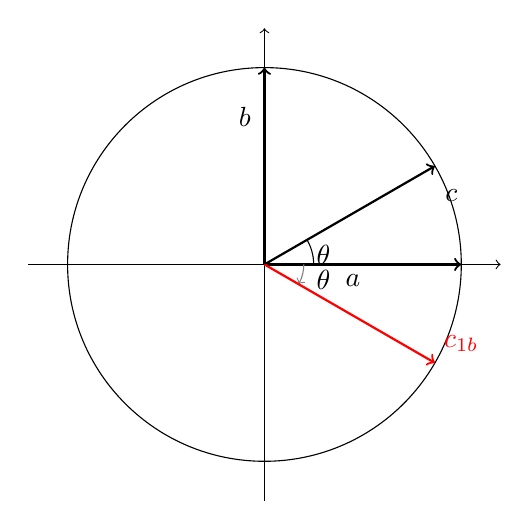
\begin{tikzpicture}[scale=2.5]

    % Draw coordinate axes
    \draw[->] (-1.2, 0) -- (1.2, 0); % x-axis
    \draw[->] (0, -1.2) -- (0, 1.2); % y-axis

    % Draw the unit circle
    \draw (0,0) circle(1);

    % Main vector c (black)
    \draw[->, thick] (0,0) -- (0.866,0.5);
    \node at (0.95,0.35) {$c$};

    % Projection on x-axis (a)
    \draw[->, thick] (0,0) -- (1,0);
    \node at (0.45,-0.08) {$a$};

    % Projection on y-axis (b)
    \draw[->, thick] (0,0) -- (0,1);
    \node at (-0.1,0.75) {$b$};

    % First angle theta
    \draw (0.25,0) arc[start angle=0,end angle=30,radius=0.25];
    \node at (0.3,0.05) {$\theta$};

    % Second angle theta (for red vector)
    \draw[gray, ->] (0.2,0) arc[start angle=0,end angle=-30,radius=0.2];
    \node at (0.3,-0.08) {$\theta$};

    % Red vector c_{1b}
    \draw[->, thick, red] (0,0) -- (0.866,-0.5);
    \node[red] at (1.0,-0.4) {$c_{1b}$};

\end{tikzpicture}
    \caption{Der Zustand des Systems nach der ersten Teil der erste Iteration}
    \label{fig:after-first-part-grover-three-qubits}
\end{figure}

Diese Spiegelung erfolgt in diesem Beispiel durch die Anwendung des $CCNOT$-Gatters. Allgemein jedoch lässt sich dieser Schritt der Orakelfunktion durch folgende Operation beschreiben:

$$
U_{1b} = I - 2|b\rangle \langle b|
$$

Hier steht $U_{1b}$ für die Orakelfunktion. Diese Operation kehrt ausschließlich das Vorzeichen der vertikalen Komponente des Zustandsvektors um, was genau zur beschriebenen Spiegelung führt.

Überprüfen wir nun die Wirkung dieser Formel anhand des Beispiels:

\begin{align*}
U_{1b} |c\rangle &= (I - 2|11\rangle \langle 11|) \cdot \frac{1}{2}(|00\rangle + |01\rangle + |10\rangle + |11\rangle) \\
&= \frac{1}{2} \left( |00\rangle + |01\rangle + |10\rangle + |11\rangle - 2|11\rangle \right) \\
&= \frac{1}{2} (|00\rangle + |01\rangle + |10\rangle - |11\rangle)
\end{align*}

Damit ist der erste Teil der Iteration abgeschlossen.

Nun wenden wir uns dem zweiten Teil der ersten Iteration zu. In diesem Schritt erfolgt eine weitere Spiegelung – jedoch nicht mehr an der horizontalen Achse, sondern am ursprünglichen Zustandsvektor $c$. Es lässt sich leicht erkennen, dass der neue Zustandsvektor danach dem Ausdruck

$$
\cos(3\theta)|a\rangle + \sin(3\theta)|b\rangle
$$

\noindent entspricht. Das bedeutet, der Winkel zwischen dem Vektor und der horizontalen Achse ist nun $3\theta$. Der Zustand wurde also weiter in Richtung des gesuchten Basiszustands $|b\rangle$ gedreht.

\begin{figure}[H]
    \centering
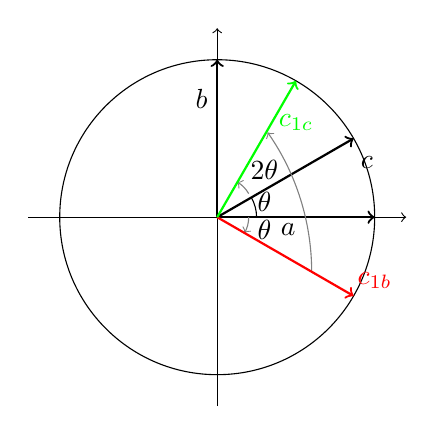
\begin{tikzpicture}[scale=2]

    % Draw coordinate axes
    \draw[->] (-1.2, 0) -- (1.2, 0); % x-axis
    \draw[->] (0, -1.2) -- (0, 1.2); % y-axis

    % Draw the unit circle
    \draw (0,0) circle(1);

    % Main vector c (black)
    \draw[->, thick] (0,0) -- (0.866,0.5);
    \node at (0.95,0.35) {$c$};

    % Projection on x-axis (a)
    \draw[->, thick] (0,0) -- (1,0);
    \node at (0.45,-0.08) {$a$};

    % Projection on y-axis (b)
    \draw[->, thick] (0,0) -- (0,1);
    \node at (-0.1,0.75) {$b$};

    % First angle theta
    \draw (0.25,0) arc[start angle=0,end angle=30,radius=0.25];
    \node at (0.3,0.1) {$\theta$};

    % Second angle theta (for red vector)
    \draw[gray, ->] (0.2,0) arc[start angle=0,end angle=-30,radius=0.2];
    \node at (0.3,-0.08) {$\theta$};

    % Third angle theta (for red vector)
    \draw[gray, ->] (0.2,0.15) arc[start angle=30,end angle=60,radius=0.2];
    \node at (0.3,0.3) {$2\theta$};

    \draw[gray, ->] (0.6,-0.35) arc[start angle=0,end angle=35,radius=1.55];

    % Red vector c_{1b}
    \draw[->, thick, red] (0,0) -- (0.866,-0.5);
    \node[red] at (1.0,-0.4) {$c_{1b}$};

    % Green vector c_{1c}
    \draw[->, thick, green] (0,0) -- (0.5,0.866);
    \node[green] at (0.5,0.6) {$c_{1c}$};

\end{tikzpicture}
    \caption{Der Zustand des Systems nach der zweiten Teil der erste Iteration}
    \label{fig:after-second-part-grover-three-qubits}
\end{figure}
Die Operation zur Erzeugung des reflektierten Vektors $c_{1c}$ sieht wie folgt aus:

$$
U_{1c} = 2|c\rangle \langle c| - I
$$

Berechnen wir den resultierenden Vektor $c_{1c}$ für unser Beispiel:

\begin{align*}
U_{1c} |c_{1b}\rangle &= \left(2|c\rangle \langle c| - I\right) \cdot \frac{1}{2} (|00\rangle + |01\rangle + |10\rangle - |11\rangle) \\
&= |11\rangle
\end{align*}

Es fand eine Spiegelung des Zustandsvektors $|c_{1b}\rangle$ an $|c\rangle$ statt. Wenn man den Vektor $|c_{1b}\rangle$ als Linearkombination $k_1 |c\rangle + k_2 |c_{\perp}\rangle$ schreiben kann, wobei $|c_{\perp}\rangle$ senkrecht auf $|c\rangle$ steht und $k_1$, $k_2$ reelle Koeffizienten sind, dann ergibt sich der gespiegelte Vektor zu:

$$
k_1 |c\rangle - k_2 |c_{\perp}\rangle
$$

Genau dies geschieht hier: Die Komponente entlang $|c\rangle$ bleibt erhalten, während die senkrechte Komponente ihr Vorzeichen ändert. In unserer Quantenschaltung wird dieser zweite Teil der Iteration folgendermaßen implementiert:

\begin{figure}[h!]
    \centering
    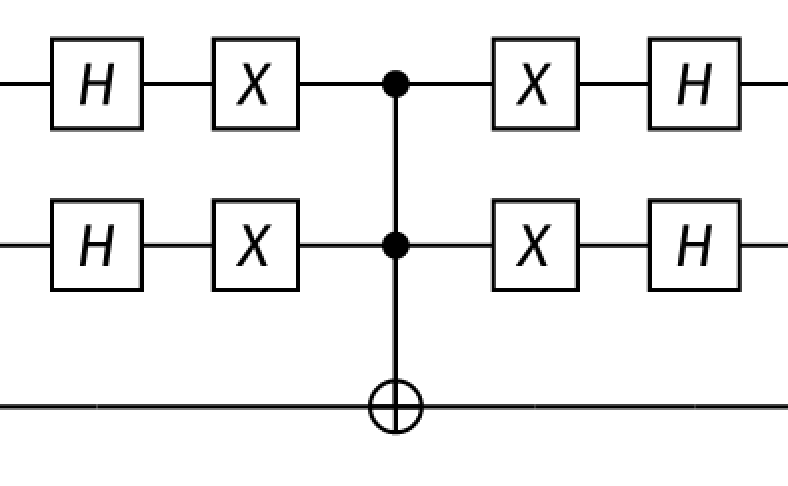
\includegraphics[width=0.4\textwidth]{images/basic-algorithms/grover-2-iteration.png}
    \caption{Zweite Iteration - $U_{1c}$}
    \label{fig:grover-second-iteration}
\end{figure}

Zunächst wird der Hadamard-Operator auf den ersten und zweiten Qubit angewendet. Dies vereinfacht unsere Aufgabe erheblich, da die Reflexion des Zustandsvektors nun nicht mehr relativ zum Superpositionszustand $\frac{1}{2}(|00\rangle + |01\rangle + |10\rangle + |11\rangle)$ erfolgen muss, sondern relativ zum Zustand $|00\rangle$.

Um die Spiegelung durchzuführen, müssten wir eigentlich allen Zuständen außer dem Nullzustand ein negatives Vorzeichen zuweisen. Stattdessen nutzen wir jedoch einen Trick: Wir versehen lediglich den Zustand $|00\rangle$ mit einem Minuszeichen und lassen alle übrigen Superpositionszustände unverändert. Dies erreichen wir durch eine gezielte Abfolge von Gattern: zuerst $X$-Gatter, dann ein $CCNOT$-Gatter, und danach wird die Transformation durch Umkehr der Schritte rückgängig gemacht – also erneut $X$-Gatter und anschließend Hadamard-Gatter.

Aufgrund dieses Tricks (Negation nur des Nullzustands) ergibt sich in unserem Beispiel mit zwei Qubits nicht $|11\rangle$, sondern $-|11\rangle$ als Ergebnis – abgesehen von einer globalen Phase. Dies ist jedoch unproblematisch, da sich die globale Phase beim Messen nicht auswirkt und wir den gesuchten Index trotzdem korrekt erhalten.

Aus der Darstellung auf dem Einheitskreis, die den Zustand des Systems nach der zweiten Hälfte der ersten Iteration veranschaulicht, wird deutlich, dass der Zustandsvektor mit jeder weiteren Iteration der Vertikalen näherkommt. In unserem konkreten Fall beträgt der Winkel zwischen Zustandsvektor und Horizontaler nach Abschluss der ersten Iteration bereits $3\theta$, was genau dem gewünschten Winkel $\frac{\pi}{2}$ entspricht.

Im allgemeinen Fall ergibt sich der Winkel nach $t$ Iterationen zu:

$$
(2t + 1)\theta \approx \frac{\pi}{2}
$$

Daraus lässt sich die erforderliche Anzahl an Iterationen für den Grover-Algorithmus bestimmen. Wenn $t$ groß ist und $K = 1$ (für $K > 1$ ist der Schluss analog), wird der Winkel $\theta$ sehr klein. Daher kann man $\theta$ durch $\sin{\theta}$ ersetzen, und es gilt näherungsweise:

$$
\theta \approx \sin{\theta} = \frac{1}{\sqrt{N}}
$$

Daraus folgt:

$$
(2t + 1) \cdot \frac{1}{\sqrt{N}} \approx \frac{\pi}{2}
$$

Wenn man die Eins im Term $(2t + 1)$ vernachlässigt (für große $t$ zulässig), erhält man:

$$
t \approx \frac{\pi \sqrt{N}}{4}
$$

Wie wir bereits gesehen haben, besteht jede Iteration aus zwei Schritten. Der erste Schritt ist die Reflexion nach unten an der Horizontalen. Der zweite Schritt ist die Reflexion nach oben an der ursprünglichen Richtung, also am Vektor $c$. Dabei wird der Zustandsvektor stets auf einen größeren Winkel nach oben reflektiert als der Winkel der vorherigen Spiegelung nach unten. Genau dadurch nähert sich der Vektor bei jeder Iteration schrittweise der Vertikalen.\\

Wir haben ein Beispiel für die Anwendung des Grover-Algorithmus betrachtet. Im nächsten Kapitel werden wir uns mit der Zeitkomplexität beschäftigen und erläutern, warum dieser Algorithmus trotz der Anzahl an Iterationen dennoch schneller ist als klassische Suchalgorithmen.


\subsection{Komplexitätsanalyse}
Der Grover‐Algorithmus durchsucht eine unstrukturierte Datenbank der Größe \(N\) mithilfe eines Quantenorakels in \(\Theta(N)\) Orakelaufrufen. Anders ausgedrückt: Während die klassische Vollsuche im Mittel \(\Theta(N)\) Prüfungen erfordert, reduziert Grover die Zahl der notwendigen Prüfungen auf etwa $\frac{\pi}{4}\,\sqrt{N}\ $ das heißt auf die Quadratwurzel der Datenbankgröße.

Aus Sicht der Komplexitätstheorie bezeichnet man die Eingangsgröße mit \(n\), so dass $N = 2^n$.
Die Laufzeit des Grover‐Algorithmus lässt sich daher durch  
$O\bigl(2^{n/2}\bigr)$ beschreiben. Obwohl dies gegenüber dem klassischen \(O(2^n)\) einen erheblichen quadratischen Gewinn darstellt, wächst der Algorithmus bei zunehmender Zahl der Suchbits weiterhin exponentiell.

Die untere Schranke aus der Arbeit von Bennett–Bernstein–Brassard–Vazirani (BBBV96 referenz) zeigt, dass kein Quantenalgorithmus im Black‐Box‐Modell mit weniger als  
\[
\Omega(\sqrt{N})
\]  
Orakelaufrufen auskommen kann. Damit ist der Grover‐Algorithmus in diesem Modell asymptotisch optimal: Ohne zusätzliche Struktur in der Datenbank lässt sich kein suprakquadratischer (etwa exponentieller) Vorteil erzielen.  


\section{Klassifikation von Algorithmen nach Zeitkomplexität}

Im Rahmen der theoretischen Informatik werden Entscheidungsprobleme nach der zur Lösung benötigten Zeit in verschiedene Klassen eingeordnet. Dabei interessiert insbesondere, welche Probleme auf einem klassischen bzw. quantenmechanischen Modell in polynomieller Zeit lösbar sind, und wie sich diese Klassen zueinander verhalten.\\

Zunächst versteht man unter der Klasse \(\mathbf{P}\) jene Probleme, für die es deterministische Algorithmen gibt, die auf einem klassischen Computer in polynomieller Zeit laufen. Formal heißt das: Ein Problem liegt in \(\mathbf{P}\), wenn es einen Algorithmus gibt, dessen Laufzeit durch einen Polynomausdruck \(O(n^k)\) für eine feste Konstante \(k\) beschränkt ist, wobei \(n\) die Eingabegröße bezeichnet. Probleme aus \(\mathbf{P}\) gelten als praktisch effizient lösbar, sofern der Exponent \(k\) nicht zu groß wird.\\

Die Klasse \(\mathbf{NP}\) (nondeterministic polynomial time) umfasst diejenigen Entscheidungsprobleme, bei denen eine etwaige Lösung auf einem klassischen Computer in polynomieller Zeit verifizierbar ist, auch wenn ein deterministischer polynomieller Lösungsalgorithmus bislang unbekannt ist. Ein typisches Beispiel ist das Teilmengen-Summen-Problem: Legt man dem Algorithmus als „Zertifikat“ eine vermutete Teilmenge vor, so kann man in \(O(n)\) bzw. \(O(n\log n)\) Zeit nachprüfen, ob die Summe den Zielwert ergibt.\\

Innerhalb von \(\mathbf{NP}\) existieren die \(\mathbf{NP}\)-\emph{vollständigen} Probleme (\(\mathbf{NP}\)\emph{-complete}), die zu den schwierigsten \(\mathbf{NP}\)-Problemen zählen. Ein Problem \(L\) ist genau dann \(\mathbf{NP}\)-vollständig, wenn \(L\in\mathbf{NP}\) und jedes andere Problem aus \(\mathbf{NP}\) in polynomieller Zeit auf \(L\) reduziert werden kann. Die berühmte \textsc{Clique}-Frage oder das \textsc{3-SAT}-Problem sind klassische Vertreter dieser Klasse. Gelingt es, eines dieser Probleme in polynomieller Zeit zu lösen, so hätte man damit einen polynomiellen Algorithmus für alle \(\mathbf{NP}\)-Probleme.\\

Die Klasse der \(\mathbf{NP}\)-\emph{harten} Probleme (\(\mathbf{NP}\)\emph{-hard}) enthält solche Probleme, auf die sich beliebige \(\mathbf{NP}\)-Probleme in polynomieller Zeit reduzieren lassen. Im Gegensatz zu \(\mathbf{NP}\)-vollständigen Problemen müssen \(\mathbf{NP}\)-harte Probleme selbst nicht in \(\mathbf{NP}\) liegen und können etwa gar nicht entscheidbar sein oder nur in exponentieller Zeit verifizierbar sein.\\

Wenn man zusätzlich zur deterministischen Rechenmaschine Zufallsbits zulässt und die Wahrscheinlichkeit, die richtige Entscheidung zu treffen, für positive und negative Instanzen jeweils oberhalb eines festen Schwellwerts (typischerweise \(>1/2\)) liegt, definiert man die Klasse \(\mathbf{BPP}\) (bounded‑error probabilistic polynomial time). Probleme in \(\mathbf{BPP}\) lassen sich mit Monte‑Carlo‑Algorithmen in polynomieller Zeit mit beliebig kleiner Fehlerrate lösen.\\

Der quantenmechanische Gegenpart zu \(\mathbf{BPP}\) ist die Klasse \(\mathbf{BQP}\) (bounded‑error quantum polynomial time). Hierbei kann ein Quantenalgorithmus für ein Problem in polynomieller Zeit auf einem Quantencomputer mit hoher Wahrscheinlichkeit das korrekte Ergebnis liefern. Ein bekanntes Beispiel ist die Ganzzahlfaktorzerlegung großer Zahlen mittels Shor’s Algorithmus, der das hierfür klassische \(\mathbf{NP}\)-Problem in polynomieller Zeit auf einem Quantencomputer löst.

\begin{figure}[h]
  \centering
  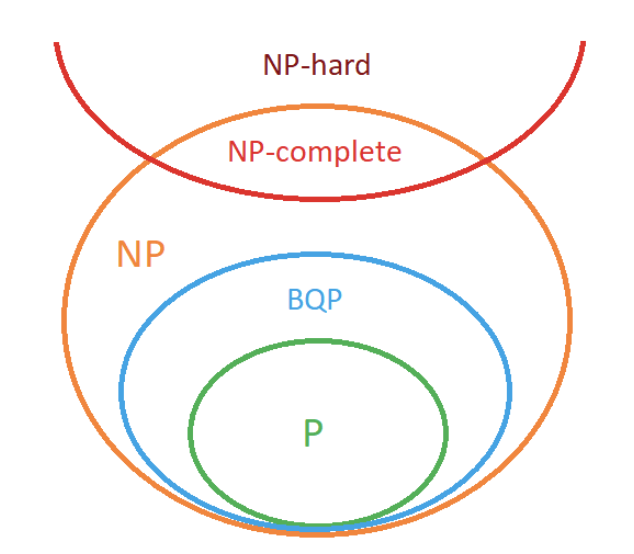
\includegraphics[width=0.7\textwidth]{images/basic-algorithms/problem-classes.png}
  \caption{Übersicht der wichtigsten Zeitkomplexitätsklassen: \(\mathbf{P}\subseteq \mathbf{BQP}\subseteq \mathbf{NP}\subseteq \mathbf{NP}\text{-hard}\) und die Lage von \(\mathbf{NP}\)-complete Problemen innerhalb von \(\mathbf{NP}\).}
  \label{fig:problem_classes}
\end{figure}

Abschließend lässt sich festhalten, dass die Frage, ob \(\mathbf{P}=\mathbf{NP}\) gilt, zu den bedeutendsten offenen Problemen der Informatik zählt. Auch der Vergleich zwischen klassischen und quantenmechanischen Modellen, speziell die Vermutung \(\mathbf{P}\subsetneq \mathbf{BQP}\subseteq \mathbf{NP}\), prägt die Forschung im Bereich effizienter Algorithmen maßgeblich.

\section{Quantum Safe Algorithmen}

\subsection*{Einleitung}

Mit der rasanten Entwicklung von Quantencomputern stehen klassische Verschlüsselungsverfahren vor einer existenziellen Bedrohung. Während heutige Systeme auf der Annahme beruhen, dass bestimmte mathematische Probleme schwer zu lösen sind, können Quantenalgorithmen wie \textit{Shor’s Algorithmus} oder \textit{Grover’s Algorithmus} diese Probleme effizient berechnen – und damit die Sicherheit brechen, auf die heutige digitale Kommunikation angewiesen ist.

Diese Bedrohung macht sogenannte \textbf{Quantum Safe Algorithmen} notwendig – kryptographische Verfahren, die auch gegen Angriffe durch leistungsfähige Quantencomputer resistent sind. Zwei Hauptansätze stehen im Zentrum der Forschung:

\begin{itemize}
  \item \textbf{Quantum Key Distribution (QKD)} – ein Verfahren, das physikalische Gesetze der Quantenmechanik nutzt, um absolut sichere Schlüsselverteilungen zu ermöglichen.
  \item \textbf{Post-Quantum Cryptography (PQC)} – klassische, quantenresistente Algorithmen, die auf heutigen Geräten ausgeführt werden können.
\end{itemize}

In diesem Kapitel werfen wir einen Blick auf beide Ansätze – und erläutern insbesondere die jüngsten Fortschritte durch das NIST (National Institute of Standards and Technology), das 2022 erste standardisierungsreife Algorithmen bekannt gegeben hat.

\subsection{Quantum Key Distribution}

Quantum Key Distribution (QKD) ermöglicht es, kryptografische Schlüssel über unsichere Kanäle zu übertragen – mit einem entscheidenden Vorteil: Jeder Abhörversuch verändert unweigerlich den Zustand der übertragenen Quanteninformation und kann somit erkannt werden.

Ein klassisches Beispiel für ein QKD-Protokoll ist das \textbf{BB84-Protokoll}, das 1984 von Bennett und Brassard entwickelt wurde und später, im Jahr 2000, von Peter W. Shor and John Preskill geprüft wurde. Es nutzt die Polarisation von Photonen, um binäre Informationen zu codieren. Der Ablauf besteht aus drei Phasen:

\begin{itemize}
  \item \textbf{Key Exchange:} Alice sendet zufällig polarisierte Photonen an Bob, der sie in zufällig gewählten Basen misst.
  \item \textbf{Key Sifting:} Über einen klassischen Kanal gleichen beide ihre verwendeten Basen ab und behalten nur die Werte, bei denen die Basen übereinstimmten.
  \item \textbf{Key Distillation:} Durch Stichproben wird geprüft, ob Abhörversuche stattfanden. Die finale Schlüssellänge ergibt sich nach dieser Bereinigung.
\end{itemize}

\noindent Neben BB84 existieren weitere bedeutende Protokolle:

\begin{itemize}
  \item \textbf{B92} (reduzierte Variante mit zwei Zuständen)
  \item \textbf{E91} (nutzte erstmals Quantenverschränkung)
  \item \textbf{BBM92}, \textbf{SARG04}, \textbf{DPS}, \textbf{COW}, \textbf{GG02} (verschiedene Weiterentwicklungen)
\end{itemize}

Für eine detaillierte Übersicht der Protokolle und deren Unterschiede siehe das Paper:
\textit{An Overview of Quantum-Safe Approaches: Quantum Key Distribution and Post-Quantum Cryptography} von Guobin Xu et al.

\subsection{Post-Quantum Cryptographie Algorithmen}

Da QKD mit hohen technischen und infrastrukturellen Anforderungen verbunden ist, setzt sich in der Praxis vor allem die \textbf{Post-Quantum Cryptography (PQC)} durch. Sie nutzt klassische Rechenverfahren, basiert jedoch auf mathematischen Problemen, die auch für Quantencomputer als schwierig gelten.

Das US-amerikanische \textbf{NIST} hat im Rahmen eines mehrjährigen Wettbewerbs Verfahren für zwei Hauptkategorien gesucht:

\begin{itemize}
  \item \textbf{Public-Key Encryption and Key Establishment (KEM)}
  \item \textbf{Digitale Signaturverfahren}
\end{itemize}

\noindent Nach mehreren Runden wählte NIST im Juli 2022 vier Algorithmen aus, die als erste Quantum Safe Standards empfohlen werden.

\noindent Für Verschlüsselung und Schlüsselaustausch nominierte NIST:

\begin{itemize}
  \item \textbf{CRYSTALS-Kyber} – 2017, J. Bos et al.
\end{itemize}

\vspace{0.5em} % optionaler vertikaler Abstand

\noindent Für digitale Signaturen nominierte NIST:

\begin{itemize}
  \item \textbf{CRYSTALS-Dilithium} – 2018, L. Ducas et al.

  \item \textbf{Falcon} – 2018, P.-A. Fouque et al.

  \item \textbf{SPHINCS+} – 2019, D. J. Bernstein et al.
\end{itemize}

\subsubsection*{CRYSTALS-Kyber}

\textbf{CRYSTALS-Kyber} ist ein \textit{lattice-basiertes Key Encapsulation Mechanism (KEM)}. Es basiert auf dem sogenannten \textit{Module Learning with Errors (MLWE)}-Problem, das auch von Quantencomputern bislang nicht effizient gelöst werden kann.

Der Algorithmus nutzt Polynomarithmetik und besteht aus drei Hauptschritten:

\begin{enumerate}
  \item \textbf{Schlüsselerzeugung:} Öffentlicher und privater Schlüssel werden erzeugt.
  \item \textbf{Encapsulation:} Ein gemeinsamer Schlüssel wird erzeugt und verschlüsselt übertragen.
  \item \textbf{Decapsulation:} Der Empfänger entschlüsselt den Schlüssel mit seinem privaten Schlüssel.
\end{enumerate}

\noindent Kyber bietet drei Sicherheitsniveaus, die sich durch unterschiedliche Parametergrößen unterscheiden und an klassische AES-Sicherheitsstufen angelehnt sind:

\begin{itemize}
  \item \textbf{Kyber-512} – Sicherheitsniveau 1 (vergleichbar mit AES-128)
  \item \textbf{Kyber-768} – Sicherheitsniveau 3 (vergleichbar mit AES-192)
  \item \textbf{Kyber-1024} – Sicherheitsniveau 5 (vergleichbar mit AES-256)
\end{itemize}

\subsubsection*{CRYSTALS-Dilithium}

\textbf{CRYSTALS-Dilithium} ist ein digitaler Signaturalgorithmus, ebenfalls basierend auf \textit{MLWE} und \textit{MSIS} (Module Short Integer Solution). Die Signaturerzeugung verwendet die \textit{Fiat-Shamir-Transformation}, die aus einem interaktiven Zero-Knowledge-Protokoll eine nicht-interaktive Signatur macht.

Dilithium bietet drei Sicherheitsniveaus:

\begin{itemize}
  \item \textbf{Dilithium2}
  \item \textbf{Dilithium3}
  \item \textbf{Dilithium5}
\end{itemize}

Die Vorteile liegen in der schnellen Verifikation, der Robustheit gegen Seitenkanalangriffe und der guten Performance. Diese Eigenschaften machen Dilithium zu einem führenden Kandidaten im Bereich der quantensicheren digitalen Signaturen.



\section{Quantum-safe Algorithmen in Kryptographie}
\subsection{Aktuelle Stand der Kryptographie}
\subsection{Vektoren in der asymmetrischen Verschlüsselung}

\section{Grover-Algorithmus für Fine-tuning von LLM}
\subsection{Idee: Transformer Architektur}
Transformer-Architekturen (Vaswani et al., 2017) bilden die Grundlage moderner großer Sprachmodelle (LLMs). Sie verwenden Self-Attention-Mechanismen, um in einem Eingabesequenz-Kontext relevante Zusammenhänge zu gewichten.\\
Ein Nachteil ist die quadratische Rechenkomplexität in der Sequenzlänge: Standard-Self-Attention erfordert $O(n^2)$ Operationen für eine Sequenz der Länge $n$. Das limitiert die Effizienz bei langen Eingaben.\\
Dieses Kapitel bietet einen Überblick über Transformer und Attention-Blöcke und ihre Rolle in LLMs, um die Ausgangsbasis für quantenbeschleunigte Ansätze zu erklären.

\subsection{Berechnung der Attention}
Gao et al. (2023) zeigten kürzlich, wie man Grover’s Suche nutzen kann, um die Attention-Matrix in Transformers effizienter zu berechnen. Sie betrachten insbesondere spärliche Attention-Matrizen und erreichen einen polynomialen Quantenvorteil gegenüber klassischen Methoden.\\
Ihr Algorithmus berechnet die relativ kleinen (sparse) Einträge der Attention-Matrix schneller, indem er Suche statt vollständiger Matrixmultiplikation verwendet.\\
Solche Quanten-Transformer sind ein aktives Forschungsthema: Sie könnten zukünftig helfen, die Rechenzeit von LLMs zu reduzieren, indem sie die Aufmerksamkeitsschichten quantenbeschleunigt umsetzen.



\printbibliography
